\documentclass[oneside,12pt,a4paper]{report}
\usepackage{babelbib}
\usepackage{puconline}
\selectlanguage{brazil}

%----------------------------------------------------------------
% Para inserção de figuras.
\usepackage{graphicx}
% Utilize a opção 'pdftex' se você estiver usando o pdflatex (que
% permite figuras em formatos como .jpg ou .png)
%\usepackage[pdftex]{graphicx}

% Para tabelas com elementos ocupando mais de uma linha
\usepackage{multirow}
% Para frações na mesma linha (ex. ⅓).
\usepackage{nicefrac}
% Para inserir figuras lado a lado.
% \usepackage{subfigure}
% Para formatar algoritmos.
% A opção [algo2e] é necessária para evitar conflitos
% com as definições da classe.
%\usepackage[algo2e]{algorithm2e}
\usepackage{algorithmic}
% Um float do tipo algoritmo. No momento
% este pacote é incompatível com a classe.
%\usepackage{algorithm}
\usepackage{amssymb}

\usepackage{fancyhdr}
\pagestyle{fancy}
\fancyhf{}
\fancyhead[RE]{\leftmark}
\fancyhead[LO]{\rightmark}
\fancyfoot[RO,LE]{\thepage}
\fancypagestyle{plain}{%  the preset of fancyhdr
    \fancyhf{} % clear all header and footer fields
    \fancyfoot[C]{\textbf{\thepage}} % except the center
    \renewcommand{\headrulewidth}{0pt}
    \renewcommand{\footrulewidth}{0pt}}





%


\fancyhead[LEO]{

\includegraphics[height=20mm]{fig/puc-online.png}
}

\fancyfoot[LEO]{

\includegraphics[scale=0.24]{fig/rodape-puconline.png}
}
\definecolor{pucrs-dark-blue}{rgb}{0,0.4,0.7}
\definecolor{pucrs-light-blue}{rgb}{0.43,0.81,0.96}
\newcommand{\note}[1]{{\color{red} {#1}}}
\definecolor{cadetblue}{rgb}{0.37, 0.62, 0.63}
\fancypagestyle{plain}{}
\newcommand{\bbleidpp}{}
\begin{document}


\begin{minipage}{16cm}
\centering
\begin{center}
{\textbf{TEMPLATE PARA ENTREGA DO PROJETO DA DISCIPLINA}}\\
{\textbf{Projeto em Business Intelligence e Analytics}}\\
{Fase 1}
\end{center}
\end{minipage}
\vspace{0.5cm}

\colorbox{pucrs-dark-blue}{\textcolor{white}{\textbf{Nome do estudante: Victor Moraes Zucchetti}}}

\chapter{Introdução}\label{chap:intro}

O agronegócio brasileiro constitui um dos pilares fundamentais da economia nacional. Segundo dados do do Centro de Estudos Avançados em Economia Aplicada (CEPEA-Esalq/USP) e da Confederação da Agricultura e Pecuária do Brasil (CNA), o setor responde por aproximadamente 25\% do Produto Interno Bruto (PIB) do país e por mais de 40\% das exportações brasileiras. Nesse ecossistema, o crédito rural desempenha um papel estruturante: é o principal instrumento de financiamento da produção agropecuária, viabilizando a aquisição de insumos, máquinas e equipamentos, a implantação de culturas e a adoção de inovações tecnológicas que sustentam a competitividade do Brasil nos mercados globais de commodities agrícolas.

O marco institucional do crédito rural no Brasil remonta à Lei n.º 4.829, de 1965, que institucionalizou o crédito rural como instrumento de política pública para o desenvolvimento do setor agropecuário. Ao longo das décadas seguintes, esse sistema expandiu-se significativamente, sendo operado tanto por instituições financeiras públicas — como o Banco do Brasil, BNDES e bancos cooperativos vinculados ao Sistema OCB — quanto por bancos privados, com recursos canalizados por meio e instrumentos como o Plano Safra e demais programas governamentais de incentivo à agricultura (e.g. Programa Nacional de Fortalecimento da Agricultura Familiar — PRONAF, Moderfrota, etc).

Não obstante a relevância estratégica do setor, o ingresso de novas instituições financeiras no mercado de crédito rural apresenta desafios de ordem técnica e informacional que distinguem esse segmento do crédito corporativo e pessoal convencional. A natureza diferenciada da atividade agrícola — caracterizada por ciclos produtivos longos, sazonalidade climática, volatilidade de preços de commodities, etc — cria uma assimetria de informação, dificultando o processo de avaliação de risco e precificação do crédito. Em particular, a ausência de um portfólio histórico interno no segmento rural impede a calibração de modelos de crédito tradicionais de risco baseados em dados comportamentais próprios.

Diante desse cenário, o Sistema de Operações do Crédito Rural e do Proagro (SICOR), mantido pelo Banco Central do Brasil (BACEN), emerge como um recurso analítico viável para a construção de modelos de crédito rural. O SICOR consolida, de forma granular, informações sobre todas as operações de crédito rural contratadas pelas instituições financeiras atuantes no país, abrangendo dados sobre atividade financiada, safra, finalidade da operação, modalidade, volume contratado, inadimplência e localização geográfica do mutuário. O acesso público a esses microdados regulatórios permite que novos entrantes no mercado de crédito rural construam conhecimento analítico sobre o perfil de risco setorial sem depender de uma base histórica própria.

Este projeto propõe, portanto, o desenvolvimento de um ecossistema de Business Intelligence (BI) e Analytics e de um modelo preditivo agnóstico de risco de crédito rural, estruturado sobre os dados públicos do SICOR, para subsidiar uma instituição financeira em sua estratégia de entrada e originação ao segmento do agronegócio. A abordagem analítica proposta está fundamentada na transformação dos dados disponíveis em inteligência de negócio para tomada de decissões estruturadas, contribuindo tanto para a sustentabilidade do negócio quanto para o avanço das práticas de analytics aplicado em finanças agrícolas.

\chapter{Referencial Teórico} \label{chap:referencial}

\section{Business Intelligence e Analytics}

Business Intelligence (BI) pode ser defino como um conjunto de processos, arquiteturas, tecnologias e ferramentas destinados a transformar dados brutos em informações estruturadas, trazendo um contexto analítico para apoiar a tomada de decisões estratégicas em diferentes níveis organizacionais \cite{kimball&ross2013}. A infraestrutura de BI tipicamente compreende um pipeline de dados que move informações para ambientes de análise — data warehouses ou data lakes — onde são integradas, limpas e modeladas em esquemas dimensionais ou relacionais, facilitando a consulta e exploração por meio de ferramentas de visualização, dashboards e relatórios gerenciais.

Analytics, por sua vez, abrange um contínuo analítico mais amplo, que \cite{davenport&jeanne2007} organizam em quatro níveis progressivos de sotisficação:
\begin{itemize}
    \item[(i)] \textbf{Analytics Descritivo} — voltado para a síntese do que aconteceu por meio de relatórios e visualizações históricas;
    \item[(ii)] \textbf{Analytics Diagnóstico} — orientado à investigação das causas de eventos observados;
    \item[(iii)] \textbf{Analytics Preditivo} — emprega modelos estatísticos e de aprendizagem de máquina para estimar probabilidades de ocorrências futuras;
    \item[(iv)] \textbf{Analytics Prescritivo} — recomenda ações ótimas com base nos modelos preditivos construídos.
\end{itemize}
No contexto financeiro, o Analytics Preditivo tem sido o nível de maior aplicação prática, especialmente em modelagem de risco de crédito, detecção de fraudes e gestão de portfólios.

\section{Modelagem de Risco de Crédito}

O risco de crédito, de forma abrangente, refere-se à probabilidade de uma contraparte não honrar suas obrigações financeiras contratuais, resultando em perdas para o credor. Os principais componentes do risco de crédito, conforme estabelecido pelos Acordos de Basileia (\cite{bcbs2004}), incluem:
\begin{itemize}
    \item[(i)]  \textbf{Probabilidade de \textit{Default} (PD)} — mensura a chance de um cliente inadimplir em um horizonte de tempo específico;
    \item[(ii)] \textbf{Perda Dado o \textit{Default} (\textit{Loss Given Default} - LGD)} — representa a fração do valor exposto que não será recuperada em caso de inadimplência.
    \item[(iii)] \textbf{Exposição no Momento do \textit{Default} (\textit{Exposure at Default} - EAD)} — quantifica o valor em risco no momento do evento de inadimplência.
    \item[]
\end{itemize}

A modelagem quantitativa do risco de crédito tem raízes no trabalho de \cite{altman1968}, que introduziu a aplicação de análise discriminante múltipla para prever falências corporativas a partir de indicadores financeiros. Subsequentemente, \cite{merton1974} desenvolveu um modelo estrutural ancorado na teoria de precificação de opções, no qual o \textit{default} de uma empresa ocorre quando o valor de seus ativos cai abaixo do valor de suas dívidas — modelo que fundamenta uma geração de abordagens baseadas no valor de mercado das empresas. Essas contribuições fundacionais estabeleceram as bases teóricas para o que viria a se tornar o \textit{credit scoring} moderno.

O \textit{credit scoring} é caracterizado pela construção de modelos estatísticos que atribuem escores numéricos a tomadores de crédito com base em suas características observáveis, constituindo a abordagem dominante para discriminar bons e maus pagadores no crédito de varejo e empresarial (\cite{siddiqi2006}). Os métodos aplicados variam desde a regressão logística — amplamente adotado pela sua interpretabilidade e aceitação regulatória — até técnicas mais complexas como florestas aleatórias (\textit{Random Forests}), \textit{Gradient Boosting} e redes neurais (\cite{breiman2001}, \cite{friedman2001}). As abordagens de aprendizagem de máquina mais recentes têm demostrado ganhos expressivos em poder preditivo, especialmente em contextos de dados de alta dimensionalidade, mas apresentam desafios em relação à interpretabilidade e à conformidade regulatória, tema abordado com crescente relevância no setor financeiro.

Embora o arcabouco de Basileia (\cite{bcbs2004}) defina o risco de crédito em termos de PD, LGD e EAD, este projeto restringe-se a modelagem da Probabilidade de \textit{Default} (PD). A escolha decorre da natureza dos microdados do SICOR, organizados por operação e adequados a estimativa da PD em nível de segmento/operação, e não da idoneidade individual do tomador como em um \textit{bureau} de crédito. A estimativa da LGD e EAD fica indicada como extensão futura.

\subsection{Modelos de Risco Agnósticos}

Denomina-se agnóstico, neste trabalho, o modelo de risco construido sem dependência de histórico comportamental interno do tomador, calibrado a partir de dados externos e regulatórios que descrevem a operacao, o segmento e o ambiente macro-setorial. Tal abordagem responde ao problema de \textit{cold-start} enfrentado por instituições entrantes, nas quais a assimetria de informação (\cite{akerlof1970}, \cite{stiglitz1981}) impede o uso de \textit{scorecards} convencionais baseados em comportamento próprio (\cite{hand&henley1997}). Cabe distinguir, nesse sentido, o agnóstico quanto a origem dos dados, do conceito técnico de interpretabilidade \textit{model-agnostic} (\cite{lundberg&lee2017}), empregado adiante para explicar modelos não-lineares.

\subsection{Modelos de Regressão Logística}

A regressão logística modela a probabilidade de inadimplência como uma função logística de uma combinação linear das variáveis explicativas, produzindo estimativas de PD no intervalo (0,1). Sua ampla adoção em \textit{credit scoring} decorre da interpretabilidade dos coeficientes e da aceitação regulatória (\cite{hand&henley1997}, \cite{thomasetal2002}), o que a torna referência natural como modelo interpretável em aplicações de crédito (\cite{siddiqi2006}). Neste projeto, ela é empregada como benchmark interpretável intermediário entre o modelo de referência naive e modelos não-lineares de maior capacidade preditiva.

\section{Crédito Rural}

O crédito rural foi institucionalizado pela Lei nº 4.829/1965, que estruturou o Sistema Nacional de Credito Rural (SNCR). Suas condicoes operacionais — modalidades (custeio, investimento, comercializacao e industrializacao), fontes (recursos controlados e livres) e programas (Plano Safra, Pronaf, entre outros) — são normatizadas pelo Manual de Credito Rural (MCR) do Banco Central. A garantia da atividade agropecuária opera por meio do Proagro. A literatura de financas agricolas (\cite{barry&ellinger2011}, \cite{turvey1991}) destaca que esse segmento exige variáveis específicas — ciclo produtivo, clima e preços de \textit{commodities} — distintas das do crédito comercial convencional.

\section{SICOR - Bacen}

O Banco Central do Brasil (Bacen) tem como atribuição institucional a regulação e supervisão do Sistema Financeiro Nacional (SFN), incluindo a normatização e o monitoramento das operações das operações de crédito rural. Por meio da Resolução n.º 4.696, de 2021 e do Manual de Crédito Rural (MCR), o Bacen exige que as instituições financeiras reportem, de forma padronizada por meio do SICOR, todas as operações de crédito rural contratadas no terrtório nacional. Os microdados do SICOR abrangem uma gama de variáveis como: CPF/CNPJ do beneficiário, município e estado, tipo de empreendimento (cultura, atividade ou produto financiado), safra, finalidade da operação (custeio, investimento, comercialização ou industrialização), valor contratado, prazo da operação, taxa de juros, e ocorrências de solicitações de seguro Proagro ou de inadimplência.

Essa base de dados, publicamente disponibilizada  para acesso no portal de Dados Abertos do Bacen, representa uma das fontes mais abrangentes de microdados estruturados sobre crédito rual no Brasil, cobrindo operações a partir do ano de 2013. Seu uso para fins acadêmicos e de inteligência de negócios é subutilizado em relação ao seu potencial analítico. A disponibilidade, granularidade e a cobertura temporal desses dados fazem do SICOR um ativo informacional de primeira ordem para a construção de modelos de risco agnóstico.

\chapter{Revisão da Literatura} \label{sec:revisao}

\section{Métodos de Modelagem de Risco de Crédito}

A literatura sobre modelagem de risco de crédito evoluiu substancialmente ao longo das últimas décadas. O trabalho seminal de \cite{hand&henley1997} revisou sistematicamente os métodos de classificação aplicados ao \textit{credit scoring}, comparando regressão logística, análise discriminante e k-vizinhos mais próximos (\textit{k-Nearest Neighbors} — k-NN), concluindo que a regressão logística oferece um melhor equilíbrio entre poder preditivo e interpretabilidade. \cite{thomasetal2002} consolidaram em obra de referência os métodos quantitativos para \textit{credit scoring} aplicáveis a portfólios de varejo e empresarial, abordando tanto a modelagem estatística quanto os aspectos de implementação operacional.

Com o avanço do aprendizado de máquina, os métodos \textit{ensemble}, ganharam poeminência nas aplicações de crédito. \cite{breiman2001} propôs o algoritmo \textit{Random Forest}, que constrói múltiplas árvores de decisão descorrelacionadas e agrega suas previsões por votação ou média, demonstrando alta robustez contra overfitting e elevada capacidade preditiva em datasets de alta dimensionalidade. \cite{friedman2001} desenvolveu o framework de \textit{Gradient Boosting}, que se tornou a base para implementações de grande impacto como o \textit{XGBoost} \cite{chen&guestrin2016}, amplamente utilizado em competições de modelagem de crédito e na indústria financeira global por sua escalabilidade e precisão.

No contexto específico do crédito rural, \cite{turvey1991} explorou a aplicação de \textit{credit scoring} a empréstimos agropecuários, identificando os desafios particulares desse segmento: variabilidade climática, dependência de ciclos de preços de commodities e a natureza cíclica do processo produtivo agrícola. \cite{barry&ellinger2011} discutem como as finanças agrícolas lidam com estruturas de risco distintas do crédito comercial convencional, exigindo variáveis específicas vinculadas à produção agrícola, ciclo operavional , condições de mercado e fatores climáticos.

Mais recentemente, a literatura tem abordado o desafio da interpretabilidade em modelos de aprendizado de máquina aplicados ao risco de crédito. \cite{lundberg&lee2017} propuseram o \textit{framework SHAP} (\textit{SHapley Additive exPlanations}), fundamentado na teoria dos jogos cooperativos, para interpretar as previsões de modelos complexos por meio da decomposição aditiva da contribuição de cada variável. O SHAP tem sido crescentemente adotado no setor financeiro para conciliar o poder preditivo de modelos complexos com a necessidade regulatória de explicabilidade das decisões de crédito.

\section{Dados Abertos e Regulatórios para Crédito Rural}

O uso de dados abertos e regulatórios para a análise de risco de crédito rural e a previsão de inadimplência é uma área em expansão tanto na literatura acadêmica quanto nas práticas de mercado. Em âmbito internacional, estudos têm explorado o uso de dados de sistemas oficiais de seguro agrícola, registro de crédito regulatórios e variáveis macroeconômicas para construir modelos que estimam o risco sem a necessidade de dados comportamentais próprios dos tomadores \cite{barry&ellinger2011}. Essa abordagem é especialmente relevante para novos entrantes e \textit{fintechs} de crédito rural, que carecem de bases históricas internas suficientes para a calibração de modelos convencionais de \textit{credit scoring}.

No contexto brasileiro, os microdados do SICOR representam uma fonte singular para esse tipo de análise. O Bacen, por meio de seus Anuários Estatísticos, documenta sistematicamente o panorama estatístico de originação, inadimplência e distribuição do crédito rural por cultura e região, estabelecendo uma base de referência empírica para o setor. Estudos baseados nessas estatísticas têm identificado padrões de inadimplência diferenciada entre culturas, regiões e safras, apontando para a forte influência de eventos climáticos adverosos (secas, geadas, etc.) e de ciclos de preços de \textit{commodities} nos índices de \textit{default}.

A integração de variáveis setoriais — como atividade, finalidade do financiamento e porte do tomador — com variáveis macroeconômicas — como câmbio, taxa Selic e Plano Safra, preços de \textit{commodities} e índices de produção agrícola — tem demostrado potencial para aumentar substancialmente a capacidade preditiva de modelos agnósticos. Essa abordagem encontra respaldo na literatura de modelagem de portfólio de crédito, que reconhece a importância dos fatores sistémicos e setoriais na determinação da probabilidade de \textit{default} \cite{thomasetal2002}. A disponibilidade pública e a cobertura temporal do SICOR posicionam esse dados como um ativo analítico de alto valor para estratégias \textit{data-driven} de entrada no mercado de crédito rural.

\chapter{Plano de Trabalho} \label{cha:plano}


\section{Descrição do Problema}

A instituição financeira objeto deste projeto pretende expandir seu portfólio de produtos por meio de oferta de crédito rural a clientes do agronegócio. No entanto, diferentemente do crédito convencional — onde a análise de risco dos solicitantes é relativamente padronizada por meio de \textit{bureaus} de crédito nacionais (Serasa Experian, Boa Vista SCPC, SPC Brasil, etc.) e de históricos comportamentais internos —, o crédito rural apresenta uma avaliação de risco distinta, governada por diferenças significativas de estrutura das operações e influências externas, como condições climáticas, safras, preços de commodities, entre outros fatores.

As principais fontes de complexidade que caracterizam o problema são:
\begin{itemize}
    \item[(i)] \textbf{Assimetria de informações:} a instituição não dispõe de dados históricos interno no segmento rural e, portanto, não possui padrões de risco comportamental calibrados para essa população;
    \item[(ii)] \textbf{Volatilidade agrícola:} a renda proveniente de atividades agrícolas é dependente de fatores climáticos (regime de chuvas, temperatura, geadas, secas, etc.), de ciclo de preços de \textit{commodities} e de características específicas de cada atividade agropecuária;
    \item[(iii)] \textbf{Heterogeneidade regional:} o Brasil possui dimensões continentais com realidades muito distintas em termos de clima, solo e outros fatores que influenciam a produção agropecuária, gerando perfis de risco diferenciados que modelos genéricos podem apresentar dificuldades para capturar;
    \item[(iv)] \textbf{Especificidade regulatória:} o crédito rural é submetido a um arcabouço normativo com regras específicas de taxas de juros, subvenções e programas de seguro (Proagro) que influenciam o comportamento de inadimplência e devem ser considerados na modelagem de risco.
\end{itemize}

Essas características tornam o desafio de modelar o risco de crédito rural mais complexo. O desafio central do projeto é, portanto: \textbf{\textit{Como construir um modelo preditivo de risco de crédito aplicável à originação de crédito rural, em um contexto de ausência de dados comportamentais próprios, utilizando microdados regulatórios públicos do SICOR/Bacen como fundamento analítico?}}

\section{Hipóteses}

A partir da descrição do problema, formulam-se as seguintes hipóteses de trabalho:
\begin{itemize}
    \item[\textbf{H1:}] A taxa de inadimplência das operações de crédito rural varia significativamente entre atividades agropecuárias, finalidades do financiamento e safras, refletindo a influência diferencial de eventos climáticos e de ciclos de mercado sobre o perfil de risco de crédito de cada segmento.
    \item[\textbf{H2:}] Um modelo preditivo de risco de crédito construido a partir de microdados do SICOR, enriquecidos com variáveis macroeconômicas, setorias e climáticas externas apresenta capacidade preditiva e discriminatória estatisticamente superior a um modelo de referência baseado exclusivamente em taxas históricas de inadimplência.
\end{itemize}

O teste dessas hipóteses fornecerá evidências empíricas sobre a estrutura do risco de crédito rural no Brasil e sobre a viabilidade científica do modelo agnóstico proposto, contribuindo tanto para os objetivos de negócio da instituição quanto para o conhecimento em relação à finanças agrícolas.

\section{Objetivos}

\subsection{Objetivo Geral}

Desenvolver um ecossistema de Business Intelligence e Analytics e um modelo preditivo agnóstico de risco de crédito rural, fundamentado em microdados públicos do Sistema de Operações do Crédito Rural e do Proagro (SICOR/Bacen), capaz de subsidiar a tomada de decisão para apoiar a originação de crédito rural em uma instituição financeira em fase de entrada no mercado, superando os desafios de ausência de dados comportamentais internos e complexidade do ambiente agrícola.

\subsection{Objetivos Específicos}

\begin{itemize}
    \item[\textbf{OE1:}] Construir um pipeline de dados robusto e escalável para ingestão, processamento e análise de microdados do SICOR, integrando fontes de dados externas relevantes (climáticas, macroeconômicas, setoriais) para enriquecer a base analítica.
    \item[\textbf{OE2:}] Realizar uma análise exploratória detalhada dos dados do SICOR para identificar padrões, tendências e relações entre variáveis que influenciam o risco de crédito rural, com foco em segmentação por atividade agropecuária, finalidade do financiamento, safra de originação, região geográfica, etc.
    \item[\textbf{OE3:}] Desenvolver e validar um modelo preditivo de risco de crédito rural utilizando técnicas de aprendizagem de máquina, comparando seu desempenho preditivo e discriminatório com um modelo de referência baseado em taxas históricas de inadimplência.
    \item[\textbf{OE4:}] Criar um dashboard interativo de Business Intelligence para visualização e monitoramento dos indicadores de risco de crédito rural, permitindo a análise dinâmica por diferentes segmentos e facilitando a tomada de decisão para a originação de crédito.
\end{itemize}

\section{Atividades e Cronograma}

O projeto está estruturado com atividades alinhadas aos objetivos específicos, com um cronograma previsto para execução ao longo de três meses (abril a junho de 2026):

\begin{itemize}
    \item[(i)] Revisão bibliográfica e definição do framework analítico;
    \item[(ii)] Extração dos dados do SICOR e avaliação da qualidade dos dados;
    \item[(iii)] Design e implementação do pipeline de ingestão e processamento dos dados (ETL/ELT);
    \item[(iv)] Análise exploratória dos dados (EDA) — originação, volumes, inadimplência por atividade e safra, etc.;
    \item[(v)] Integração de variáveis externas (climáticas, macroeconômicas, setoriais) para enriquecimento da base analítica;
    \item[(vi)] Desenvolvimento e treinamento do modelo de risco de crédito;
    \item[(vii)] Validação e comparação do modelo preditivo com o modelo de referência;
    \item[(viii)] Construção dos dashboards de BI (panorama de originação e risco);
    \item[(ix)] Síntese dos resultados, elaboração do relatório final e apresentação executiva dos resultados.
\end{itemize}

\begin{table}[]
    \caption{Cronograma de Atividades para 2026.}
    \label{tab:cronograma}
    \centering
    \begin{tabular}{c|c|c|c}
        Atividade & Abril & Maio & Junho  \\ \hline
         & & & \\ \hline
         1 & \checkmark &  & \\ \hline
         2 & \checkmark &  & \\ \hline
         3 & \checkmark & \checkmark & \\ \hline
         4 & & \checkmark & \\ \hline
         5 & & \checkmark & \checkmark\\ \hline
         6 & & \checkmark & \checkmark\\ \hline
         7 & & \checkmark & \checkmark\\ \hline
         8 & & & \checkmark\\ \hline
         9 & & & \checkmark\\ \hline
    \end{tabular}
\end{table}

\section{Metodologia}

A metodologia deste projeto segue uma abordagem quantitativa, estruturada em cinco etapas principais:

\subsection{Etapa 1: Coleta de Dados}

Os microdados públicos do SICOR/Bacen serão extraídos diretamente do portal de Dados Abertos do Bacen, cobrindo a série histórica disponível (2013-até o momento). As tabelas relevantes incluem: operações de crédito rural (origem, atividade, finalidade, volume financiado, região, etc.) e registro de pagamentos (inadimplência, datas de vencimento, etc.). De forma complementar, serão coletadas variáveis externas de fontes como IBGE-SIDRA (área plantada, produtividade), Bacen-SGS (taxa Selic, PIB) e CEPEA-Esalq/USP (preços de commodities).

\subsection{Etapa 2: Pipeline de Processamento de Dados}

Um pipeline de processamento será implementado compreendendo:
\begin{itemize}
    \item[(i)] extração dos dados brutos do SICOR e das fontes externas;
    \item[(ii)] transformação, com padronização de chaves de integração, tratamento de dados faltantes, codificação de variáveis categóricas, etc.;
    \item[(iii)] carga em um ambiente de analítico estruturado (data warehouse ou data lake).
\end{itemize}
O pipeline será desenvolvido em Python (cudf, DuckDB), documentado e versionado com Git, seguindo boas práticas de engenharia de dados para garantir reprodutibilidade e escalabilidade.

\subsection{Etapa 3: Análise Exploratória de Dados (EDA)}

Estatísticas descritivas serão calculadas para as principais variáveis de interesse. Será realizado também um diagnóstico do panorama de originação e inadimplência por segmento (atividade, finalidade, safra, região). Visualizações gráficas (histogramas, boxplots, mapas de calor, etc.) serão utilizadas para identificar padrões e relações entre variáveis. A análise de correlação e testes estatísticos serão aplicados para avaliar associações significativas.

\subsection{Etapa 4: Modelagem Preditiva de Risco de Crédito}

A variável-alvo (binária: 0 = adimplente; 1 = inadimplente) será construida a partir dos registros de inadimplência no SICOR. Os modelos preditivos serão estimados em sequência crescente de complexidade, iniciando pelo modelo de referência (\textit{Naïve} baseado em taxas históricas) de inadimplência e finalizando com o modelo de aprendizado de máquina utilizando regressão logística com \textit{feature engineering} e \textit{feature selection} a partir das variáveis do SICOR e das fontes externas. A seleção e avaliação dos modelos seguirão validação cruzada com estratificação por safra agrícola, para garantir a generalização temporal e evitar \textit{data leakage}. O desempenho dos modelos será avaliado por meio das métricas de Área sob a Curva ROC (AUROC), estatística KS (\textit{Kolmogorov-Smirnov}), \textit{Brier Score} e curvas de calibração. A interpretabilidade do modelo será analisada através dos coeficientes da regressão logística (betas), avaliando a influência de cada variável no risco de crédito rural.

\subsection{Etapa 5: Desenvolvimento dos Dashboards de BI}

Os resultados estruturados serão apresentados em dashboards interativos abrangendo:
\begin{itemize}
    \item[(i)] painel de originação, com indicadores de volume financiado, número de operações, tendências por segmento, etc.;
    \item[(ii)] painel de risco, com indicadores de inadimplência por segmento, distribuição de risco, etc.
    \item[(iii)] \textit{output} de \textit{scoring} do modelo de risco.
\end{itemize}
Os dashboards serão desenvolvidos utilizando a biblioteca Streamlit, com Python, com camadas de navegação e filtros para análise dinâmica por diferentes segmentos (atividade, finalidade, safra, região, etc.). O código dos dashboards será documentado e versionado para garantir reprodutibilidade e manutenção futura.

\section{Desenho da Solução}

\begin{figure}
    \centering
    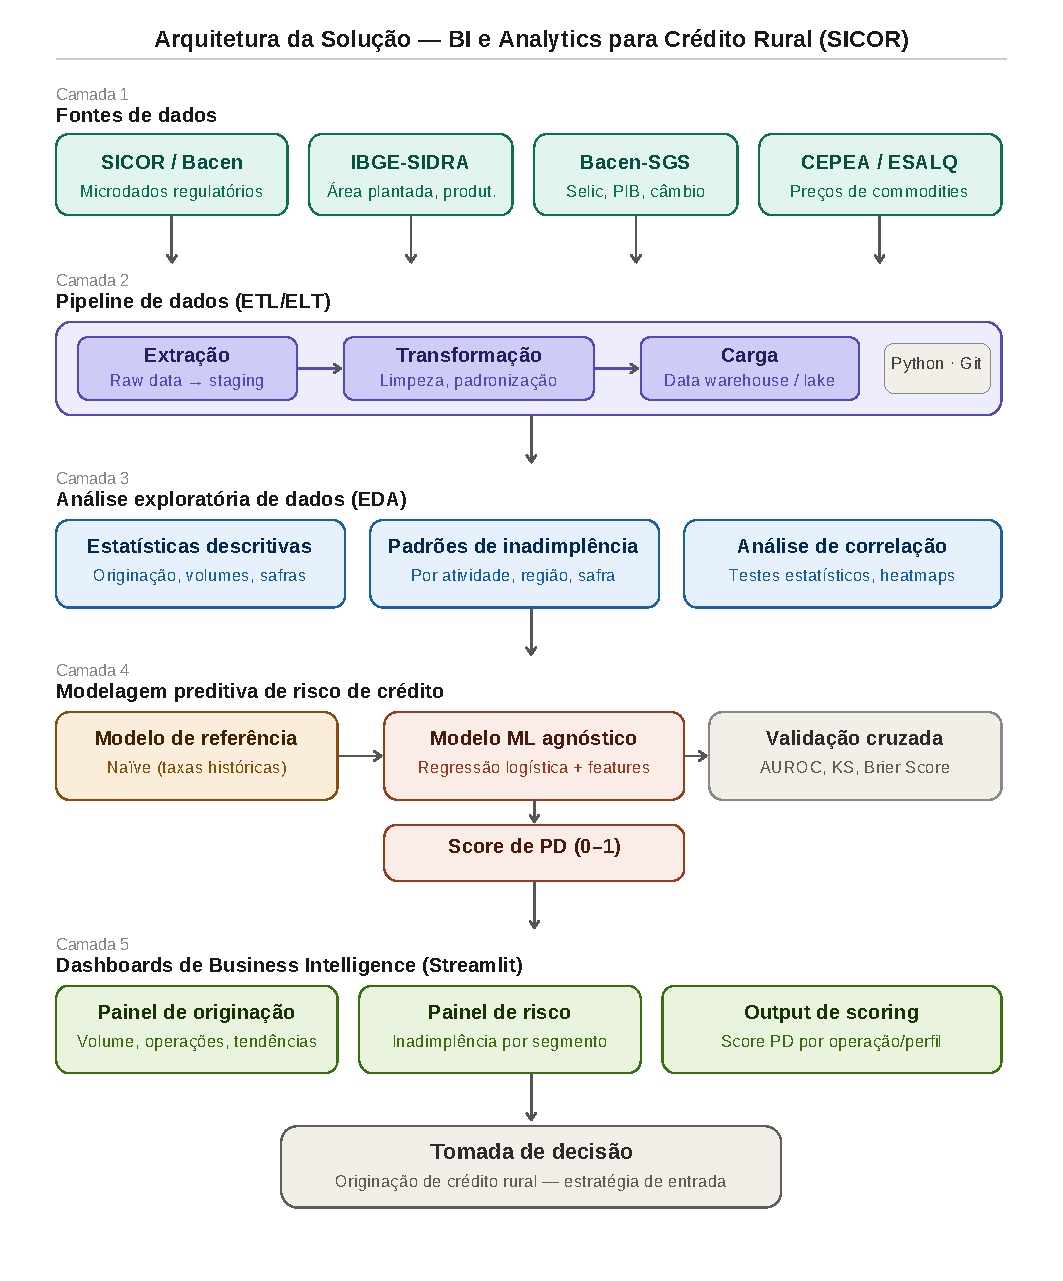
\includegraphics[scale=0.9]{fig/arquitetura_solucao_bi_credito_rural.pdf}
    \caption{Desenho da Arquitetura da Solução}
    \label{fig:desenho-solucao}
\end{figure}

A arquitetura conceitual da solução proposta segue um modelo de camadas progressivas, desde a ingestão dos dados brutos até a entrega do BI para os usuários finais, conforme ilustrado na Figura \ref{fig:desenho-solucao}.

O fluxo de dados percorre as cinco camadas de forma sequencial e rastreável, com as fontes regulatórias e setoriais sendo ingeridas, armazenadas em seu formato bruto. Posteriormente, os dados são processados e transformadas em uma base analítica estruturada, para então serem integrados a modelagem dimensional dos dados. A camada de modelagem opera sobre os dados tratados para produzir as probabilidades de \textit{default} e, por fim, estes serão disponibilizados em dashboards de BI para análise e tomada de decisão. O design modular da arquitetura garante que cada camada possa ser desenvolvida, testada, mantida e atualizada de forma independente, promovendo a escalabilidade e a flexibilidade da solução ao longo do tempo.

\chapter{Conclusão} \label{cha:conclusao}

Este projeto propõe uma solução analítica cientificamente fundamentada e aplicável para instituições financeiras que buscam ingressar no mercado de crédito rural de forma eficiente e segura, mesmo sem possuir bases de dados históricas. Ao utilizar os microdados regulatórios públicos do SICOR como fundamento analítico primário, o projeto transforma um contexto de assimetria de informação em um ambiente de decisão estruturada, demonstrando que a inteligência de dados públicos pode ser um diferencial competitivo legítimo e de alto valor estratégico.

Os impactos técnicos esperados do projeto incluem:
\begin{itemize}
    \item[(i)] Construção de um pipeline analítico reprodutível e documentado para o tratamento dos dados do SICOR, passível de manutenção e atualização à medida que novas safras agrícolas sejam incorporadas à base;
    \item[(ii)] Panorama estatístico detalhado da inadimplência por atividade, região, safra e finalidade, provendo à instituição uma visão robusta do perfil de risco dos diferentes subsegmentos do agronegócio;
    \item[(iii)] Modelo preditivo de risco de crédito rural agnóstico, validado por métricas padronizadas e interpretáveis, capaz de suportar a originação inicial de crédito rural na ausência de portfólio históricos próprio;
    \item[(iv)] Dashboard operacional de BI que traduz os insights em visualizações acessíveis e acionáveis para as equipes de crédito e de risco da instituição.
\end{itemize}

Do ponto de vista da metodologia científica, o projeto demonstra a viabilidade de construir modelos preditivos de risco de crédito a partir de dados públicos e regulatórios — uma abordagem com ampla aplicabilidade para outros segmentos financeiros onde a escassez de dados históricos constitui uma barreira de entrada relevante. A validação empírica das hipóteses formuladas contribuirá para o conhecimento a respeito do tema, especialmente em relação à capacidade de generalização dos modelos preditivos construídos a partir de dados públicos.

A convergência entre o ecossistema de BI e a modelagem preditiva de risco, ancorada em dador reais e acessíveis publicamente, posiciona este projeto como um caso de referência replicável para estratégias \textit{data-driven} no setor financeiro, contribuindo simultaneamente para o sucesso comercial da instituição, maturação das práticas de analytics aplicado a este setor e avanço do conhecimento científico em gestão de risco de crédito rural.




\bibliographystyle{formato-alpha}
%\bibliographystyle{tcc-num}
\bibliography{exemplo}


\end{document}
